
\documentclass{article}

\title{Lab 4}
\author{George Onwubuya}
\usepackage{fancyvrb}
\usepackage{minted}
\usepackage{graphicx}

\begin{document}
\maketitle

\section{Output}
\subsection{Matrix Output (m x n )}
\VerbatimInput{./convolution.sh.o558892}

\subsection{Matrix Output (m x m)}
\VerbatimInput{./convolution.sh.o560222}

 \section{Performance Analysis}
 \subsection{Rectangle Matrices (m x n)} 
 \setlength{\parindent}{1cm}
 \begin{tabular}{ |p{2.5cm}||p{2cm}|p{2cm}|p{2cm}|p{2cm}|p{2cm}|  }
 \hline
 \multicolumn{6}{|c|}{Execution Time (seconds) for Each Process } \\
 \hline
Elements(m*n) & Setting Up & DeviceVar & HostToDevice & Kernel & DeviceToHost\\
 \hline
 600 x 1000 & 0.006791 & 0.0.201096 & 0.001548 & 0.000209 & 0.001337\\
 \hline
 1200 x 2000 & 0.025171 & 0.181609  & 0.004396 & 0.000497 & 0.006667\\
 \hline
 2400 x 4000 & 0.097721 & 0.184917 & 0.020479 & 0.001661 & 0.032120\\
 \hline
 4800 x 8000 & 0.400631  & 0.183295 & 0.077317 & 0.006211 & 0.121019\\
 \hline
 9600 x 16000 & 1.571396  & 0.192857 & 0.259799 & 0.024441 & 0.475482\\
 \hline
 \end{tabular}
 \\
 \\
 \\
 \subsection{Square Matrices (m x m)}
 \begin{tabular}{ |p{2.5cm}||p{2cm}|p{2cm}|p{2cm}|p{2cm}|p{2cm}|  }
 \hline
 \multicolumn{6}{|c|}{Execution Time (seconds) for Each Process }\\
 \hline
Elements(m*m) & Setting Up & DeviceVar & HostToDevice & Kernel & DeviceToHost\\
 \hline
 1000 & 0.012148 & 0.160189 & 0.002237 & 0.000304 & 0.003576\\
 \hline
 2000 & 0.042840 & 0.147785 & 0.007397 & 0.000784 & 0.010515\\
 \hline
 4000 & 0.168949 & 0.146379 & 0.031356 & 0.002791 & 0.043496\\
 \hline
 8000 & 0.667698  & 0.147719 & 0.129577 & 0.010494 & 0.222300\\
 \hline
 16000 & 2.687160 & 0.156885 & 0.535993 & 0.041381 & 0.637439\\
 \hline 
  \end{tabular}
  
\subsection{Comments}
There is an observable increase in time for each execution subsection as the number of elements increases. The time taken to set up the problem, copy data from host to device, launch the kernel and copy from device to host increases. There is a direct proportion between the execution times and the number of elements. This observation is true both rectangle and square matrices

\section{Answers}
\subsection{C(i)}   
The floating point computation rate varies as the size of the matrices increase. The choice of matrix size was double the size of m for a series of executions in order to observe how the kernel times changed. That means a matrix with m = 2000 would scale by 4 if m is doubled, m = 4000. The kernel execution times for the matrices are shown below in the table. When the number of elements increases from 1000 to 2000, the time is scaled by 2.6, and with subsequent increases (2000, 4000, 8000 & 16000) the times are scaled by 3.6, 3.8 & 4. 
\\
\\
\\
 \setlength{\parindent}{1cm}
 \begin{tabular}{|p{3cm}||p{3cm}|}
 \hline
 \multicolumn{2}{|c|}{Kernel Execution Time (seconds)}\\
 \hline
 Elements (m x m) & Launch Kernel\\
 \hline
 1000 & 0.000304\\
 \hline
 2000 & 0.000784\\
 \hline
 4000 & 0.002791\\
 \hline
 8000 & 0.010494\\
 \hline
 16000 & 0.041381\\
 \hline
 \end{tabular}
 
\graphicspath{./Graph.png}
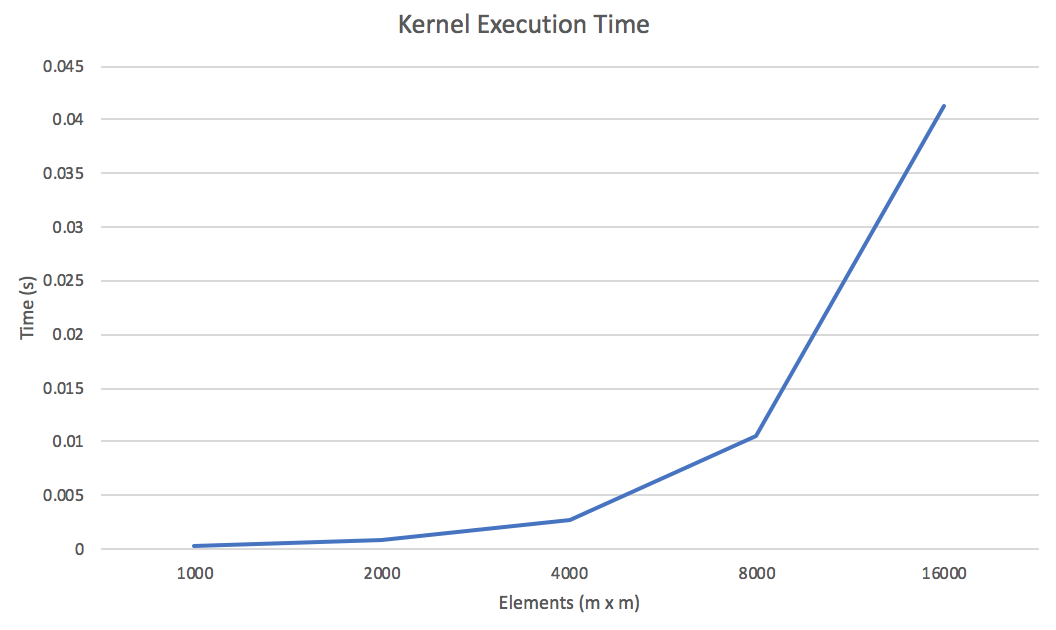
\includegraphics[width=\textwidth]{Graph}

\subsection{C(ii)}
\setlength{\parindent}{0cm}
\setlength{\parskip}{1em}
The table below shows the overhead, which is the total time spent on the GPU side as a ratio over the total execution time expressed as a \%. The amount of time spent in the GPU increases as the number of elements increase. GPU overhead accounts for more than 95\% of the total execution time
\\
\\
\\
 \setlength{\parindent}{1cm}
 \begin{tabular}{|p{3cm}||p{3cm}|p{3cm}|p{3cm}|}
 \hline
 \multicolumn{4}{|c|}{Overhead Time as a Percentage}\\
 \hline
 Elements (m x m) & Total Time & Device Time & Overhead \\
 \hline
 1000 & 0.166306 & 0.166002 & 99.81720443\\
 \hline
 2000 & 0.166481 & 0.165697 & 99.52907539\\
 \hline
 4000 & 0.224022 & 0.221231 & 98.75414022\\
 \hline
 8000 & 0.51009 & 0.499596 & 97.94271599\\
 \hline
 16000 & 1.371698 & 1.330317 & 96.98322809\\
 \hline
 \end{tabular}


\section{Main}
\inputminted[breaklines, linenos]{c}{./main.cu}

\section{Kernel}
\inputminted[breaklines, linenos]{c}{./kernel.cu}

\end{document}




